\documentclass[12pt]{article}
\usepackage[utf8]{inputenc}
\usepackage[T2A]{fontenc}
\usepackage[russian]{babel}
\usepackage{amsmath, amssymb}
\usepackage{geometry}
\usepackage{graphicx}
\usepackage{titlesec} % Для настройки заголовков
\usepackage{enumitem} % Для настройки списков
\usepackage{fancyhdr} % Для колонтитулов
\usepackage{tabularx} % Для таблиц
\usepackage{lastpage} % Для номера последней страницы



% --- НАСТРОЙКА СТИЛЯ ---
\geometry{a4paper, left=25mm, right=15mm, top=20mm, bottom=20mm, headheight=15pt}
\setlength{\parindent}{0pt} % Убираем абзацный отступ
\setlist[enumerate]{topsep=5pt, itemsep=8pt, leftmargin=25pt} % Настройка списков
\titleformat{\section}{\large\bfseries\centering}{\thesection}{1em}{} % Стиль секций

% --- КОЛОНТИТУЛЫ (со 2-й страницы) ---
\pagestyle{fancy}
\fancyhf{}
\fancyhead[L]{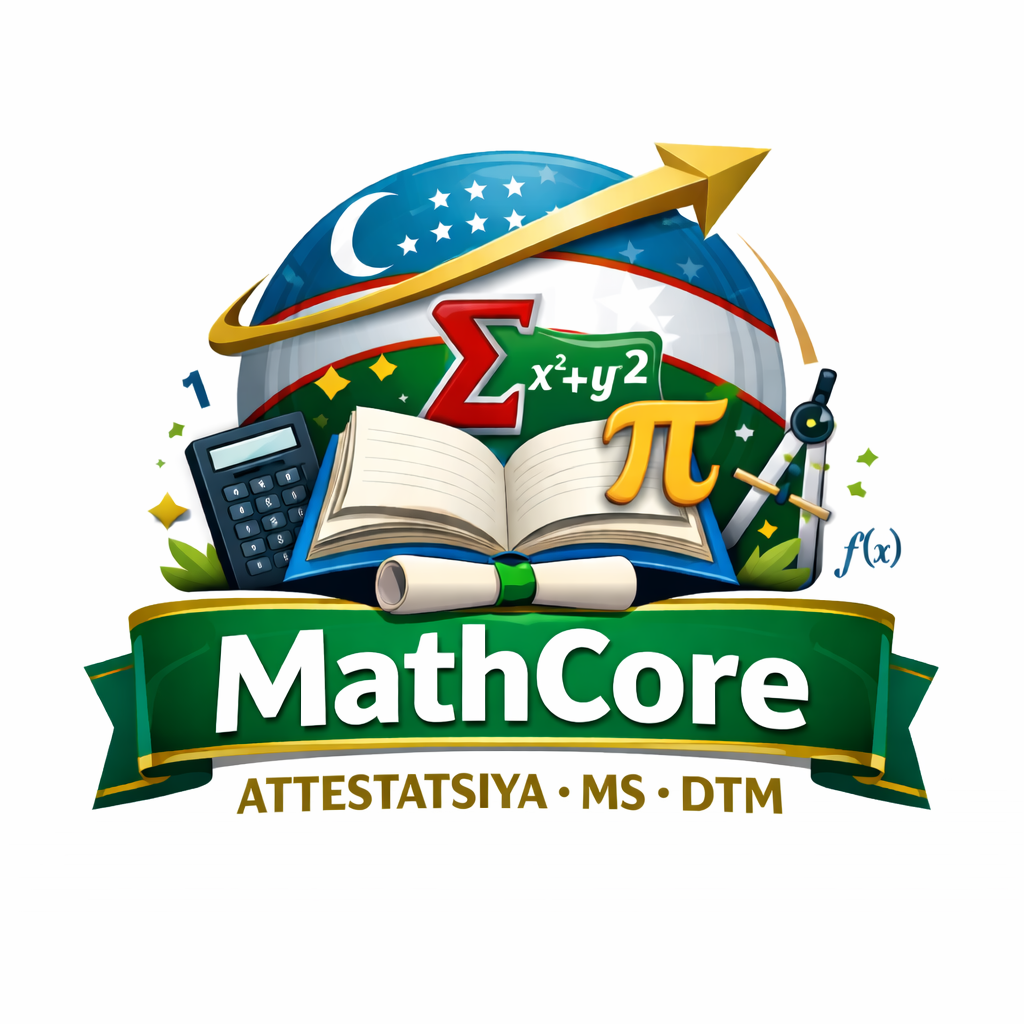
\includegraphics[height=1.1cm]{logo.png} \textbf{MathCore} | MOCK Test-1}
\fancyhead[R]{Abdunazarov M.X.}
\fancyfoot[C]{}
\renewcommand{\headrulewidth}{0.4pt}

\title{MOCK Test-1}
\author{Abdunazarov M.X.}
\date{}
\begin{document}

\maketitle
\begin{center}
  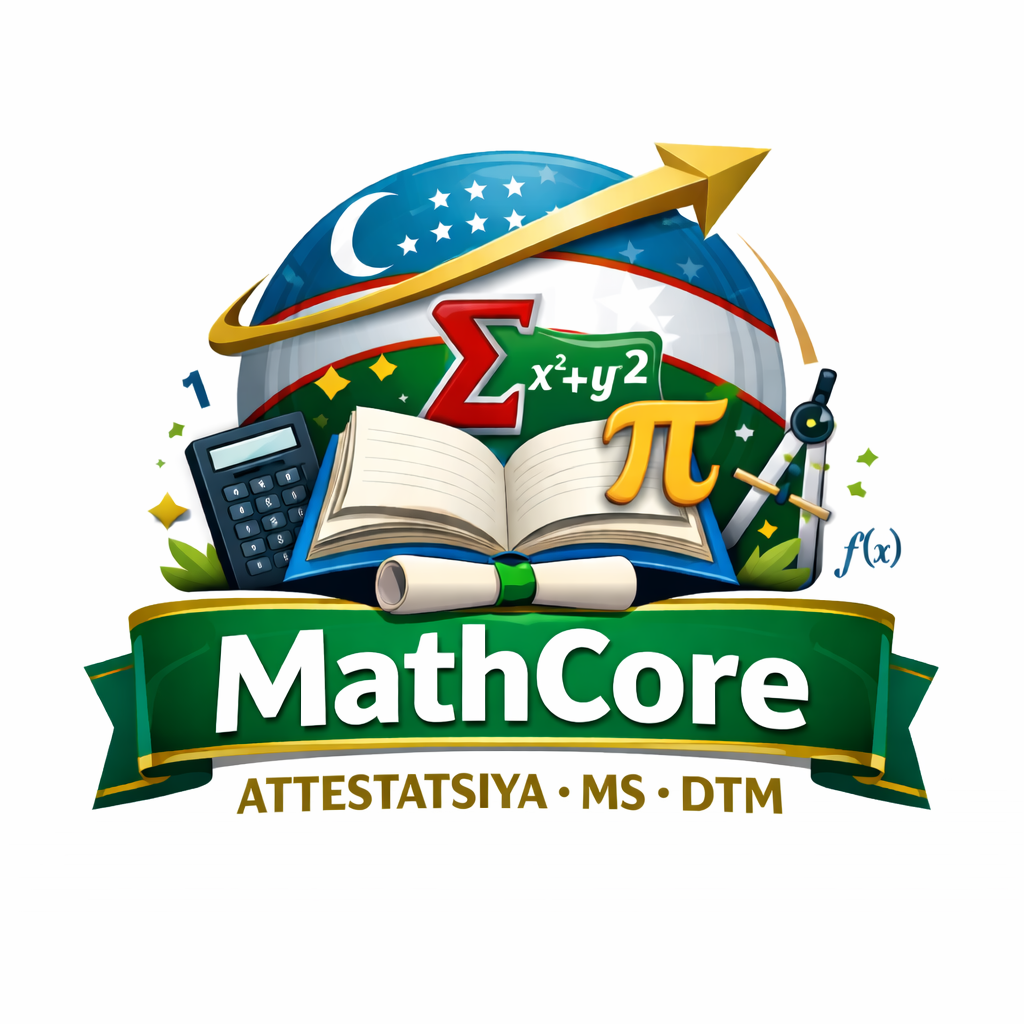
\includegraphics[width=5cm]{logo.png}
\end{center}
\begin{enumerate}

\item Если \( f(2x+1) + f(x+2) = x^2 - 5x + 3 \), найдите \( f'(3) \).
\\ A) -1,5    
B) -1    
C) 0    
D) 1
\vspace{4cm}

\item Решите дифференциальное уравнение \( \sqrt{y^2 + 1} = x y y' \).
\\ A) \( \sqrt{y^2 + 1} = \ln x + C \)    
B) \( \sqrt{y^2 + 1} = 2 \ln x + C \)    
C) \( \sqrt{y + 1} = \ln x^2 + C \)    
D) \( \sqrt{y^2 - 1} = \ln x + C \)
\vspace{4cm}

\item Найдите тупой угол между прямыми \( 5x - y + 7 = 0 \) и \( 2x - 3y + 1 = 0 \).
\\ A) 45°    
B) 60°    
C) 120°    
D) 135°
\vspace{4cm}

\item В прямой треугольной призме основания имеют стороны 6, 8, 10, а боковое ребро равно 15. Через меньшую высоту основания и боковое ребро проведено сечение. Найдите площадь сечения.
\\ A) 36    
B) 48    
C) 60    
D) 72
\vspace{4cm}

\item Если \( f(2x+1) = x^2 + 6x + 12 \), найдите значение \( f'(5) \).
\\ A) 2    
B) 5    
C) 2,5    
D) 5,5
\vspace{4cm}

\item Если \( f(x) + f'(x) = x^3 + 2x^2 + 4x + 1 \), найдите функцию \( f(x-1) \).
\\ A) \( f(x-1) = x^3 - x^2 + 6x - 5 \)    
B) \( f(x-1) = x^4 + x^3 - 6x - 5 \)    
C) \( f(x-1) = x^4 - x^3 + 6x - 5 \)    
D) \( f(x-1) = x^3 - 4x^2 + 11x - 13 \)
\vspace{4cm}

\item Найдите угол между часовой и минутной стрелками в 12:40.
\\ A) 240°    
B) 140°    
C) 160°    
D) 80°
\vspace{4cm}

\item Сумма трех последовательных нечетных чисел равна 12021. Найдите значение наименьшего из них.
\\ A) 2007    
B) 2003    
C) 4005    
D) 4013
\vspace{4cm}

\item Найдите остаток от деления числа \( 2^{2024} + 1 \) на 17.
\\ A) 1    
B) 2    
C) 16    
D) 0
\vspace{4cm}

\item Найдите остаток от деления числа \( 10^{2721} + 5 \) на 17.
\\ A) 16    
B) 15    
C) 10    
D) 14
\vspace{4cm}

\item Для двух последовательных чисел, кратных 3, m и n, выполнено НОД(m;n) + НОК(m;n) = 471. Найдите m + n.
\\ A) 36    
B) 39    
C) 75    
D) 81
\vspace{4cm}

\item Если \( \int (f'(x) - 2x) dx = 2f(x) + x^3 - x^2 \), найдите \( f'(1) \).
\\ A) 3    
B) -1    
C) 1    
D) -3
\vspace{4cm}



\item Найдите первообразную функции \( f(x) = \sin 2x \), проходящую через точку \( M(0;1) \).
\\ A) \( -\cos 2x + 2 \)    
B) \( -\frac{1}{2} \cos 2x + \frac{3}{2} \)    
C) \( \frac{1}{2} \cos 2x + \frac{1}{2} \)    
D) \( \cos 2x \)
\vspace{4cm}

\item Числа \( x_1 \) и \( x_2 \) являются корнями уравнения \( x^2 - (m + 4)x + 2m - 1 = 0 \). При сколько целых значениях m выполняется неравенство \( x_1^2 x_2 + x_1 x_2^2 \leq 0 \)?
\\ A) 2    
B) 3    
C) 4    
D) 5
\vspace{4cm}

\item Если \( 4f(x) + f(2\pi - x) = 2x^3 + 8 \), найдите \( f'(\pi) \).
\\ A) \( 6\pi^2 \)    
B) \( 3\pi^2 \)    
C) \( 2\pi^2 \)    
D) \( 4\pi^2 \)
\vspace{4cm}

\item Если \( \int f(x)dx = x^3 + 3x^2 + mx + n \) и \( f(1) = 10 \), найдите \( F(3) - F(0) \). (Здесь \( F(x) \) - первообразная функции \( f(x) \))
\\ A) 53    
B) 57    
C) 59    
D) невозможно определить
\vspace{4cm}



\item Сколько групп можно образовать, выбрав по одной птице из 3 гусей, 4 уток и 2 кур?
\\ A) 10    
B) 12    
C) 18    
D) 24
\vspace{4cm}


\item В треугольной пирамиде стороны основания равны 25, 29 и 36. Все боковые ребра образуют одинаковые углы с плоскостью основания, а высота равна 6. Найдите объем конуса, вписанного в эту пирамиду.
\\ A) 288\(\pi\)    
B) 244\(\pi\)    
C) 144\(\pi\)    
D) 128\(\pi\)
\vspace{4cm}

\item Дана треугольная пирамида с взаимно перпендикулярными ребрами, равными 5, 8, 12. Найдите объем пирамиды.
\\ A) 120    
B) 100    
C) 80    
D) 60
\vspace{4cm}





\item Дан график квадратичной функции \( y = ax^2 + bx + c \). Используя график, сравните a, b, c.
\begin{center}
    \centering
    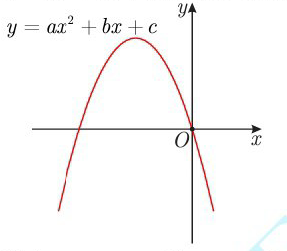
\includegraphics[width=0.5\linewidth]{6.png}
\end{center}
\\ A) \(b < a < c\)    
B) \(a < c < b\)    
C) \(b < x < a\)    
D) \(c < a < b\)
\vspace{4cm}

\item Труба A одна заполняет пустой резервуар за 6 часов, труба B одна - за 3 часа. Труба C опорожняет \( \frac{2}{3} \) резервуара за 4 часа. За сколько времени заполнится пустой резервуар, если все три трубы работают вместе?
\begin{center}
    \centering
    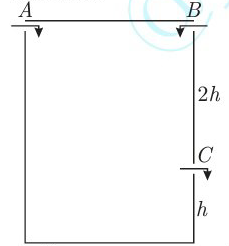
\includegraphics[width=0.5\linewidth]{7.png}
\end{center}
\\ A) \(\frac{8}{3}\)    
B) 2,5    
C) \(\frac{7}{5}\)    
D) \(\frac{9}{5}\)
\vspace{4cm}

\item Найдите объем тела, полученного вращением области, ограниченной кривыми \( y = x^2 + 1 \) и \( y = 2 \), вокруг оси Oy.
\\ A) \(\frac{\pi}{2}\)    
B) \(\frac{2\pi}{3}\)    
C) \(\frac{3\pi}{2}\)    
D) \(\pi\)
\vspace{4cm}

\item Решите дифференциальное уравнение \( y'(x + 1) = x y \).
\\ A) \( y = \frac{Ce^x}{x+1} \)    
B) \( y = \frac{Ce^x}{x-1} \)    
C) \( y = C(x+1)e^x \)    
D) \( y = C(x+1)e^{-x} \)
\vspace{4cm}

\item Радиусы маленьких окружностей равны \( r = 2 \). Найдите площадь закрашенной зеленой области.
\begin{center}
    \centering
    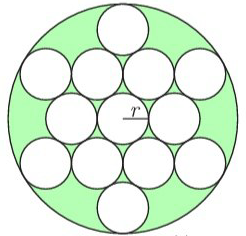
\includegraphics[width=0.5\linewidth]{8.png}
\end{center}
\\ A) \( 8\sqrt{3}\pi \)    
B) \( \frac{44}{\sqrt{3}}\pi \)    
C) \( \frac{52}{\sqrt{3}}\pi \)    
D) \( 16\sqrt{3}\pi \)
\vspace{4cm}

\item В первом сплаве отношение металлов 2:3, во втором сплаве тех же металлов отношение 3:4. В каком соотношении нужно взять эти сплавы, чтобы получить сплав с отношением металлов 11:15?
\\ A) первый сплав 5 частей, второй 21 часть    
B) первый сплав 6 частей, второй 20 частей    
C) первый сплав 7 частей, второй 19 частей    
D) первый сплав 8 частей, второй 18 частей
\vspace{4cm}

\item Если ABCD квадрат (BE = EC, AK = KB, AB = 10), найдите площадь треугольника EFG.
\begin{center}
    \centering
    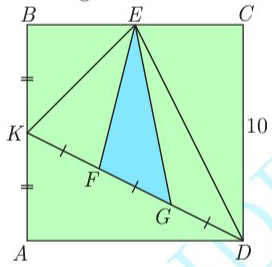
\includegraphics[width=0.5\linewidth]{9.png}
\end{center}
\\ A) 14    
B) 12,5    
C) 12    
D) \( 8\frac{1}{3} \)
\vspace{4cm}

\item Если \( P_{EDC} = 16 \) и \( AB = 15 \), найдите \( P_{ABC} \).
\begin{center}
    \centering
    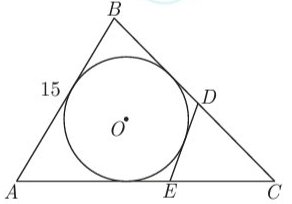
\includegraphics[width=0.5\linewidth]{11.png}
\end{center}
\\ A) 30    
B) 40    
C) 46    
D) 47
\vspace{4cm}

\item Даны четыре числа. Первые три образуют геометрическую прогрессию, последние три - арифметическую прогрессию. Сумма крайних членов равна 21, сумма двух средних равна 18. Найдите произведение всех четырех чисел.
\\ A) 3636    
B) 3838    
C) 3888    
D) 3996
\vspace{4cm}

\item Используя данные на рисунке, найдите x.
\begin{center}
    \centering
    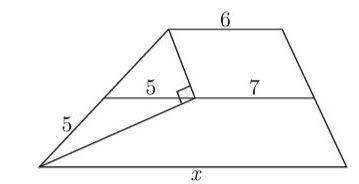
\includegraphics[width=0.5\linewidth]{12.png}
\end{center}
\\ A) 15    
B) 16    
C) 17    
D) 18
\vspace{4cm}

\item 75\% студентов знают язык A, 65\% знают язык B. Число студентов, знающих оба языка, в 3 раза больше числа студентов, не знающих ни одного языка. Какой процент студентов знают оба языка?
\\ A) 60\%    
B) 45\%    
C) 50\%    
D) 55\%
\vspace{4cm}

\item Если \( \int_{-1}^{2} x \cdot f'(x) dx = 10 \), найдите \( \int_{-1}^{2} f(x) dx \).
\begin{center}
    \centering
    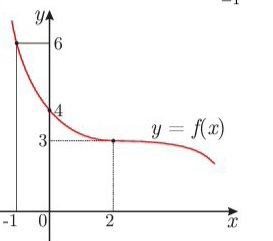
\includegraphics[width=0.5\linewidth]{13.png}
\end{center}
\\ A) 0    
B) 2    
C) 4    
D) -4
\vspace{4cm}

\item При каком значении k площадь области, ограниченной линиями \( y = k e^{\frac{x}{2}} \), \( x = 2 \), \( x = 0 \) и \( y = 0 \), равна объему тела, полученного вращением этой области вокруг оси Ox?
\\ A) \(\frac{2}{\pi(e-1)}\)    
B) \(\frac{2e}{\pi}\)    
C) \(\frac{2}{\pi(e+1)}\)    
D) \(\frac{2}{e\pi}\)
\vspace{4cm}

\item Найдите объем тела, полученного вращением области, ограниченной линиями \( y = \sqrt{x} \) и \( y = \frac{x}{2} \), вокруг оси Oy.
\\ A) \(\frac{64}{15}\pi\)    
B) 9,6\(\pi\)    
C) 9\(\pi\)    
D) \(\frac{15}{2}\pi\)
\vspace{4cm}

\item В первом случае мальчик поднимает груз с силой 2 Н, причем производная силы по высоте задана как \( \frac{dF}{dh} = \frac{1}{\sqrt{h}} + 3 + \frac{1}{h+1} \). Сколько силы (в Н) он затратит во втором случае?
\begin{center}
    \centering
    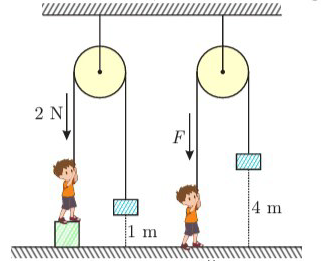
\includegraphics[width=0.5\linewidth]{14.png}
\end{center}
\\ A) 13    
B) \( 13 - \ln \frac{5}{2} \)    
C) \( 13 + \ln \frac{5}{2} \)    
D) 11,5
\vspace{4cm}

\item В пирамиде с основанием-треугольником со сторонами 25, 29, 36 и высотой 6 найдите радиус вписанной сферы.
\\ A) \(\frac{10}{3}\)    
B) \(\frac{7}{3}\)    
C) \(\frac{7}{2}\)    
D) \(\frac{8}{3}\)
\vspace{4cm}

\end{enumerate}

\end{document}